\textbf{Цель: }Получить навыки формализации и обработки информации с
использованием семантических сетей

\textbf{Задача: }Построение графа инциденций неориентированного графа

\section{Список понятий}

\begin{enumerate}
\item
  Графовая структура (абсолютное понятие) - это такая одноуровневая
  реляционная структура, объекты которой могут играть роль либо вершины,
  либо связки:

  \begin{enumerate}
  \item
    Вершина (относительное понятие, ролевое отношение);
  \item
    Связка (относительное понятие, ролевое отношение).
  \end{enumerate}

\begin{figure}[H]
  \centering
  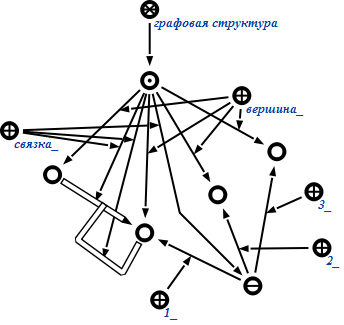
\includegraphics[scale=0.7]{images/1.png}
  \caption{Графовая структура}
\end{figure}

\item
  Графовая структура с неориентированными связками (абсолютное понятие)

  \begin{enumerate}
  \item
    Неориентированная связка (относительное понятие, ролевое отношение)
    --связка, которая задается неориентированным множеством.
  \end{enumerate}

\begin{figure}[H]
  \centering
  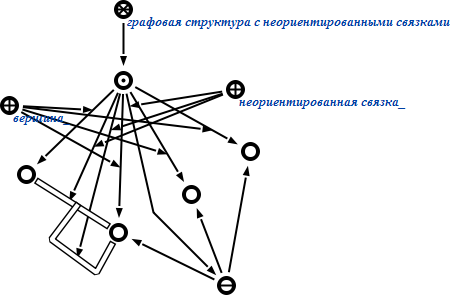
\includegraphics[scale=0.7]{images/3.png}
  \caption{Графовая структура с неориентированными связками}
\end{figure}

\item
  Граф (абсолютное понятие) -- это такой мультиграф, в котором не может
  быть кратных связок, т.е. связок у которых первый и второй компоненты
  совпадают:

\begin{figure}[H]
  \centering
  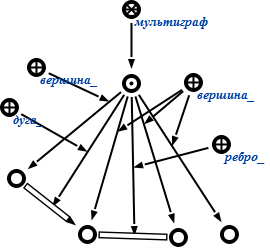
\includegraphics[scale=0.7]{images/7.png}
  \caption{Граф}
\end{figure}

\item
  Неориентированный граф (абсолютное понятие) -- это такой граф, в
  котором все связки являются ребрами:

\begin{figure}[H]
  \centering
  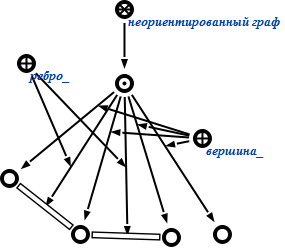
\includegraphics[scale=0.7]{images/8.png}
  \caption{Неориентированный граф}
\end{figure}

\item
Двудольный граф (абсолютное понятие) -- это граф, множество вершин которого можно разбить на две части таким образом, что каждое ребро графа соединяет какую-то вершину из одной части с какой-то вершиной другой части, то есть не существует ребра, соединяющего две вершины из одной и той же части.

\begin{figure}[H]
  \centering
  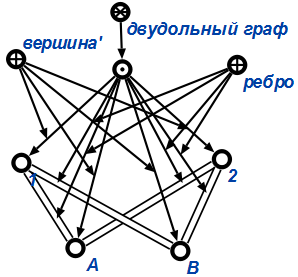
\includegraphics[scale=0.7]{images/10.png}
  \caption{Двудольный граф}
\end{figure}

\item
Граф инциденций (относительное понятие, ролевое отношение) -- двудольный граф, у которого вершины в первой доле совпадают с множеством вершин исходного графа, а вершины второй доли соответствуют ребрам исходного графа. Две вершины в графе инциденций смежны тогда и только тогда, когда соответствующие им элементы инцидентны в исходном графе.В примере ниже показан граф инциденций неориентированного графа.

\begin{figure}[H]
  \centering
  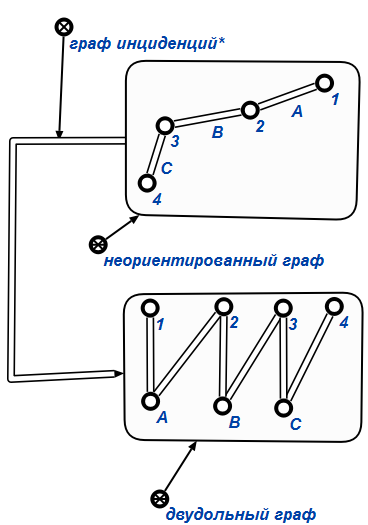
\includegraphics[scale=0.7]{images/11.png}
  \caption{Граф инциденций}
\end{figure}

\end{enumerate}

\section{Тестовые примеры}

Во всех тестах графы будет приведены в сокращенной форме со скрытыми ролями элементов графа.

\subsection{Тест 1}

\textbf{Вход:}

Необходимо построить граф инциденций неориентированного графа.

\begin{figure}[H]
  \centering
  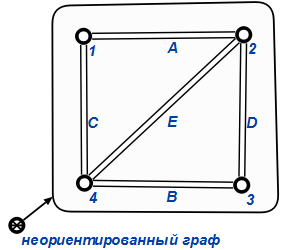
\includegraphics[scale=0.7]{images/13.png}
  \caption{Вход теста 1}
\end{figure}

\textbf{Выход:}

Будет построен граф инциденций:

\begin{figure}[H]
  \centering
  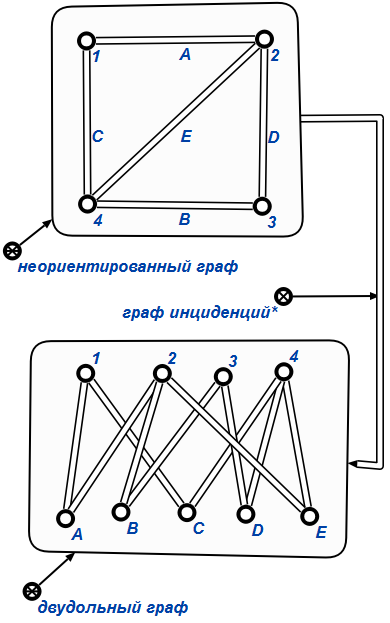
\includegraphics[scale=0.7]{images/14.png}
  \caption{Выход теста 1}
\end{figure}

\subsection{Тест 2}

\textbf{Вход:}

Необходимо построить граф инциденций неориентированного графа.

\begin{figure}[H]
  \centering
  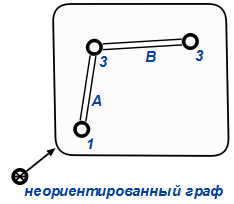
\includegraphics[scale=0.7]{images/15.png}
  \caption{Вход теста 2}
\end{figure}

\textbf{Выход:}

Будет построен граф инциденций:

\begin{figure}[H]
  \centering
  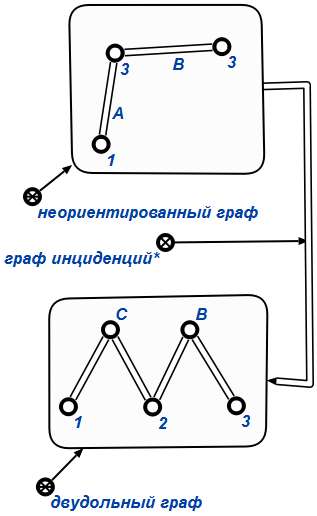
\includegraphics[scale=0.7]{images/16.png}
  \caption{Выход теста 2}
\end{figure}

\subsection{Тест 3}

\textbf{Вход:}

Необходимо построить граф инциденций неориентированного графа.

\begin{figure}[H]
  \centering
  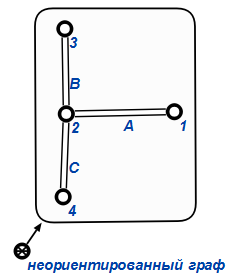
\includegraphics[scale=0.7]{images/17.png}
  \caption{Вход теста 3}
\end{figure}

\textbf{Выход:}

Будет построен граф инциденций:

\begin{figure}[H]
  \centering
  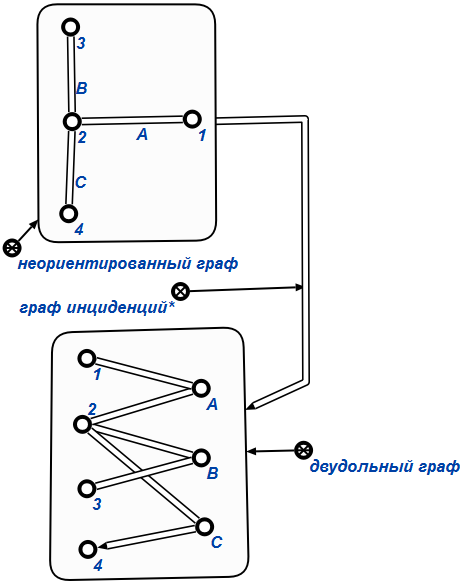
\includegraphics[scale=0.7]{images/18.png}
  \caption{Выход теста 3}
\end{figure}

\subsection{Тест 4}

\textbf{Вход:}

Необходимо построить граф инциденций неориентированного графа.

\begin{figure}[H]
  \centering
  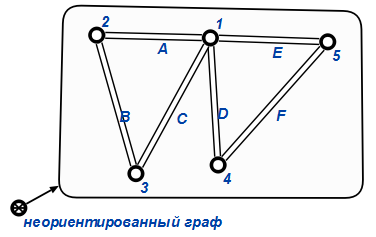
\includegraphics[scale=0.7]{images/19.png}
  \caption{Вход теста 4}
\end{figure}

\textbf{Выход:}

Будет построен граф инциденций:

\begin{figure}[H]
  \centering
  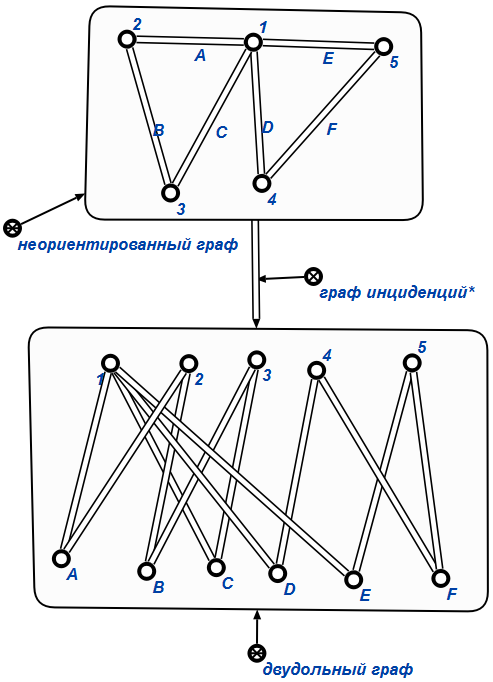
\includegraphics[scale=0.7]{images/20.png}
  \caption{Выход теста 4}
\end{figure}

\subsection{Тест 5}

\textbf{Вход:}

Необходимо построить граф инциденций неориентированного графа.

\begin{figure}[H]
  \centering
  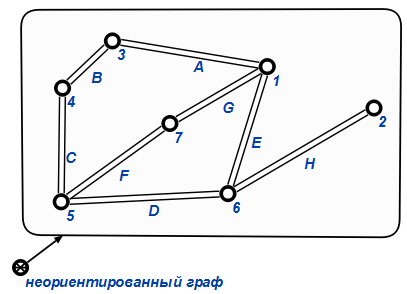
\includegraphics[scale=0.7]{images/21.png}
  \caption{Вход теста 5}
\end{figure}

\textbf{Выход:}

Будет построен граф инциденций:

\begin{figure}[H]
  \centering
  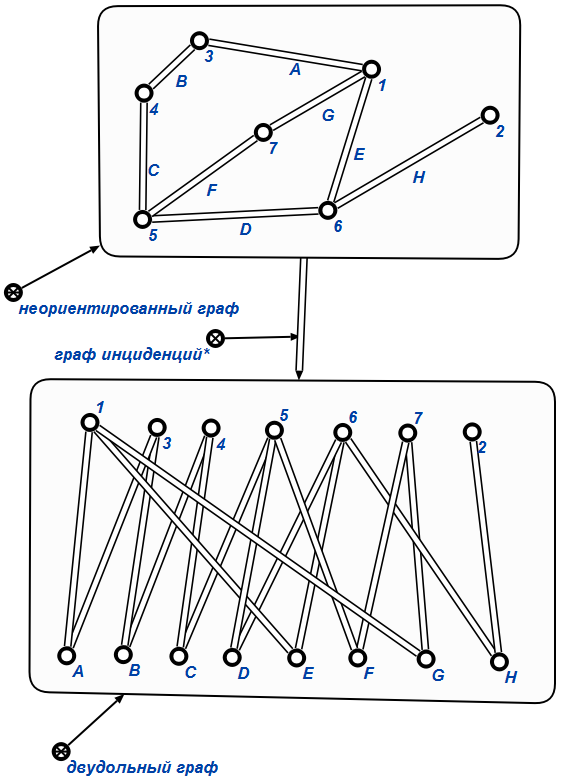
\includegraphics[scale=0.7]{images/22.png}
  \caption{Вход теста 4}
\end{figure}

\section{Пример работы алгоритма в семантической памяти}

\begin{enumerate}

\item
\textbf{Задание входного графа}
\begin{figure}[H]
  \centering
  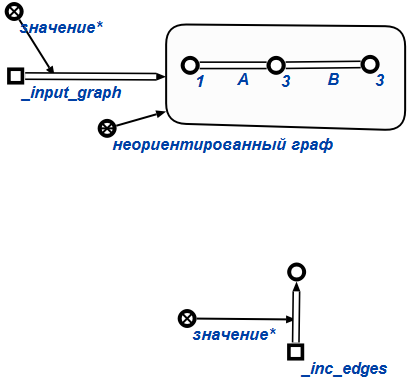
\includegraphics[scale=0.7]{algo/1.png}
  \caption{Шаг 1}
\end{figure}
\_input\_graph получит в качестве значения sc-узел неориентированного графа.
\_inc\_edges получает в качестве значения пустое множество.

\item
\textbf{ Создание множества вершин графа инцидентности}
\begin{figure}[H]
  \centering
  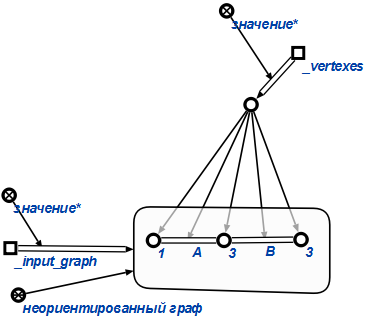
\includegraphics[scale=0.7]{algo/2.png}
  \caption{Шаг 2}
\end{figure}
Переменная \_vertexes получит в качестве значения множества вершин и ребер обрабатываемого графа.

\item
\textbf{Создание множества непроверенных ребер обрабатываемого графа}
\begin{figure}[H]
  \centering
  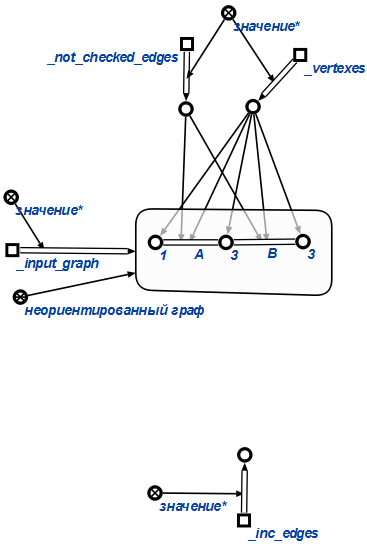
\includegraphics[scale=0.7]{algo/3.png}
  \caption{Шаг 3}
\end{figure}
Переменная\_not\_checked\_edges получит в качестве значения множество необработанных  ребер обрабатываемого графа. 

\item
\textbf{Пока есть непроверенные ребра:}

  \begin{enumerate}
   \item[1.]
   \textbf{Взятие ребра}
   \begin{figure}[H]
     \centering
     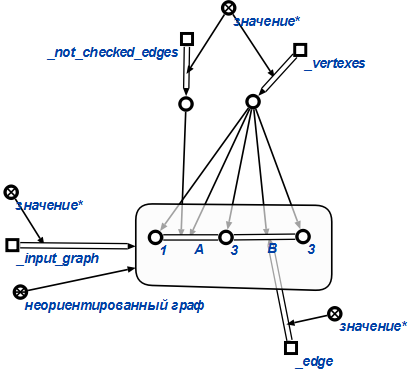
\includegraphics[scale=0.7]{algo/41.png}
     \caption{Шаг 4.1}
   \end{figure}
   Переменная \_edge получает в качестве значения ребро из множества
   \_not\_checked\_edges. Соответствующее ребро исключается и
   множества \_not\_checked\_edges.
    
   \item[2.]
   \textbf{Взятие смежных ребру вершин}
   \textbf{Взятие ребра}
   \begin{figure}[H]
     \centering
     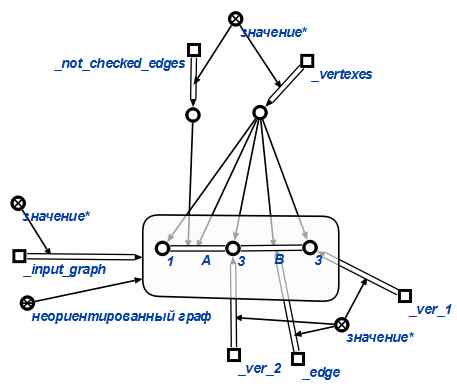
\includegraphics[scale=0.7]{algo/42.png}
     \caption{Шаг 4.2}
   \end{figure}
   Переменные \_ver\_1 и \_ver\_2 получает в качестве значений первую и вторую инцидентную ребру \_edge вершин
   
   \item[3.]
   \textbf{Создание ребра для графа инцидентности}
   \begin{figure}[H]
     \centering
     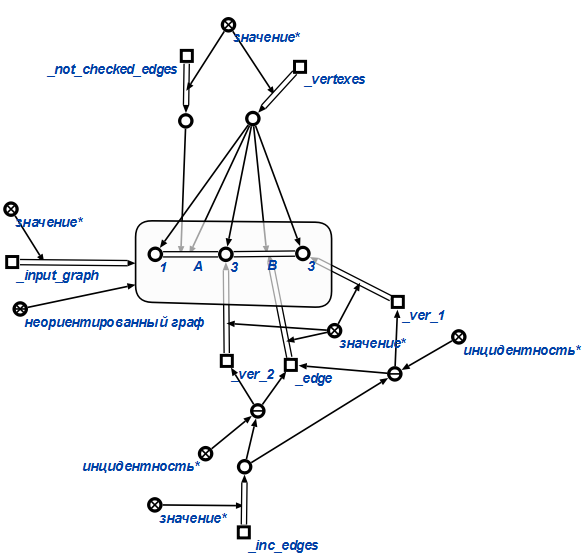
\includegraphics[scale=0.7]{algo/43.png}
     \caption{Шаг 4.3}
   \end{figure}
   В множество значений переменной \_inc\_edges добавляется отношение инцидентности между ребром \_edge и вершиной \_ver\_1
   В множество значений переменной \_inc\_edges добавляется отношение инцидентности между ребром \_edge и вершиной \_ver\_2
  \end{enumerate}

\item
\textbf{Формирование графа инцидентности}
\begin{figure}[H]
  \centering
  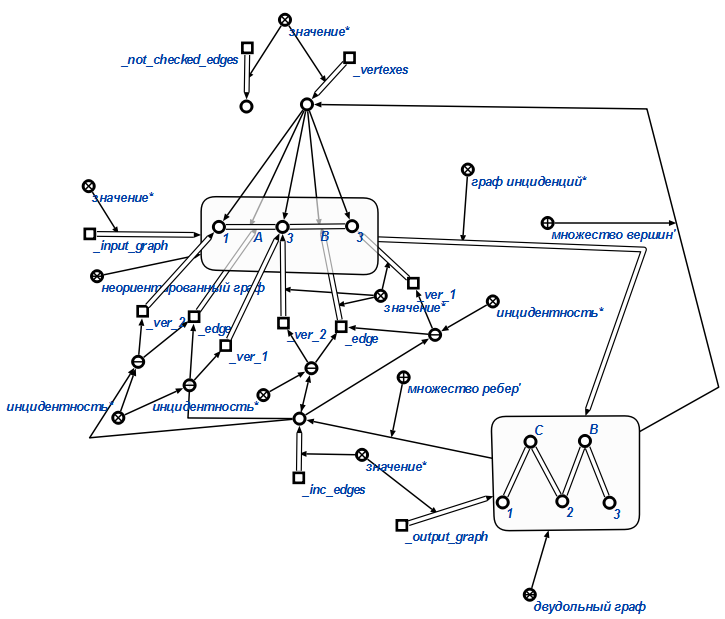
\includegraphics[scale=0.7]{algo/5.png}
  \caption{Шаг 5}
\end{figure}
Переменная \_output\_graph получит в качестве значения граф инциденций, у которого значение переменной \_inc\_edges является множеством ребер, а значение переменной \_vertexes -- множеством вершин.

\item
\textbf{Завершение работы алгоритма}
\begin{figure}[H]
  \centering
  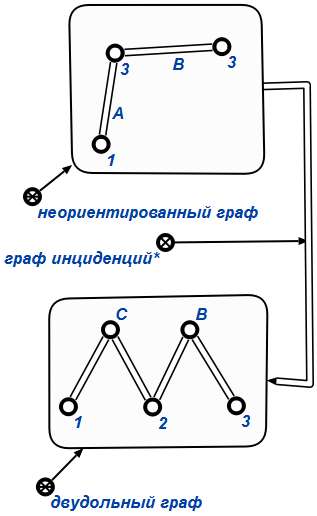
\includegraphics[scale=0.7]{images/16.png}
  \caption{Шаг 6}
\end{figure}
На данном этапе продемонстрирован результат работы алгоритма, значение переменной \_output\_graph будет возвращено в вызывающий контекст.

\end{enumerate}





















